\documentclass{beamer}

\usepackage[utf8]{inputenc}
\usepackage[T1]{fontenc}
\usepackage{tikz}
\usepackage{fontspec}
\usepackage{wrapfig}
\usepackage{float}
\usepackage{amsmath}

\usetheme{metropolis}
\usetikzlibrary{matrix}
\setmainfont[Ligatures=TeX]{Fira Sans}

\title{Pronalazak najkraćeg puta algoritmom A*}

\date{\today}

\author{Marko Lazarić\\
Voditelj: Doc. dr. sc. Marko Čupić}

\newcommand{\engl}[1]{ (engl. \emph{#1})}
\newcommand{\twocolumns}[2]{
	\begin{columns}
		\begin{column}{0.4\textwidth}
			#1
		\end{column}
		\begin{column}{0.6\textwidth}  %%<--- here
			#2
		\end{column}
	\end{columns}
}
\newcommand{\state}[2]{\textsc{Stanje}(\( #1 \), \( #2 \))}

\newcommand{\actionName}[1]{#1}
\newcommand{\upAction}{\actionName{Gore}}
\newcommand{\downAction}{\actionName{Dolje}}
\newcommand{\leftAction}{\actionName{Lijevo}}
\newcommand{\rightAction}{\actionName{Desno}}

\begin{document}
  \maketitle
  
  \section{Definicija problema}
  \begin{frame}{Početno stanje}	
  	\twocolumns{
	  \begin{figure}[H]
	  		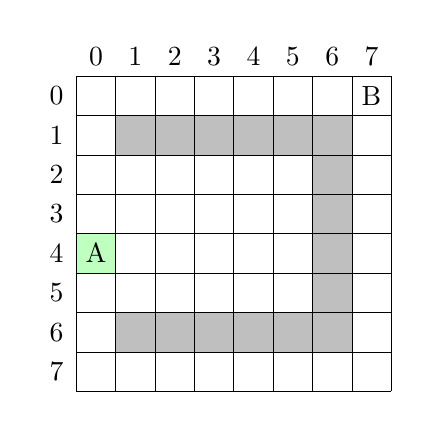
\begin{tikzpicture}
	  		\begin{scope}[xshift=-1.75cm, yshift=1.75cm, xscale=0.5, yscale=0.5]
	\fill[fill = lightgray] (1, -1) 
	  -- ++(6, 0) 
	  -- ++(0, -6) 
	  -- ++(-6, 0) 
	  -- ++(0, 1) 
	  -- ++(5, 0) 
	  -- ++(0, 4) 
	  -- ++(-5, 0) 
	  -- cycle;
	  
	\fill[fill = green!25] (0, -5) -- ++(1, 0) -- ++(0, 1) -- ++(-1, 0) -- cycle;
	
\end{scope}

\begin{scope}[xshift=0.25cm, yshift=-0.25cm]
	\draw[step=0.5cm,black,very thin] (-2,-2) grid (2,2);
\end{scope}

\matrix[matrix, matrix of nodes, nodes={anchor=center,inner sep=0pt,text width=.5cm,align=center,minimum height=.5cm}, nodes in empty cells]{
	& 0 & 1 & 2 & 3 & 4 & 5 & 6 & 7 \\
	0 &   &   &   &   &   &   &   & B \\
	1 &   &   &   &   &   &   &   &   \\
	2 &   &   &   &   &   &   &   &   \\
	3 &   &   &   &   &   &   &   &   \\
	4 & A &   &   &   &   &   &   &   \\
	5 &   &   &   &   &   &   &   &   \\
	6 &   &   &   &   &   &   &   &   \\
	7 &   &   &   &   &   &   &   &   \\};
	  		\end{tikzpicture}
	  \end{figure}
    }{
      \begin{itemize}
    	\item \emph{Početno stanje} \engl{initial state} je stanje u kojem počinje pretraživanje
      	\item U slučaju cjelobrojne rešetke, to je stanje koje sadrži "A"
      \end{itemize}
    }
  \end{frame}

  \begin{frame}{Akcije}
    \twocolumns{
    	\begin{figure}[H]
    		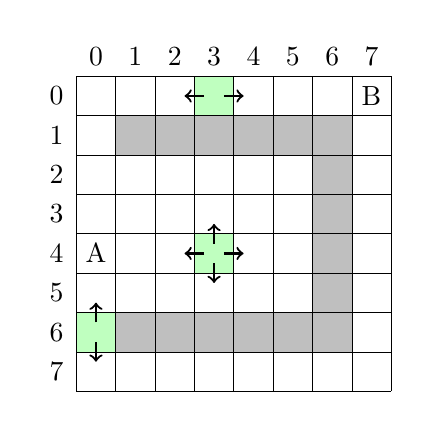
\begin{tikzpicture}
    		\begin{scope}[xshift=-1.75cm, yshift=1.75cm, xscale=0.5, yscale=0.5]
	\fill[fill = lightgray] (1, -1) 
	  -- ++(6, 0) 
	  -- ++(0, -6) 
	  -- ++(-6, 0) 
	  -- ++(0, 1) 
	  -- ++(5, 0) 
	  -- ++(0, 4) 
	  -- ++(-5, 0) 
	  -- cycle;
	  
	  \fill[fill = green!25] (3, -5) -- ++(1, 0) -- ++(0, 1) -- ++(-1, 0) -- cycle;
	  \fill[fill = green!25] (3, -1) -- ++(1, 0) -- ++(0, 1) -- ++(-1, 0) -- cycle;
	  \fill[fill = green!25] (0, -7) -- ++(1, 0) -- ++(0, 1) -- ++(-1, 0) -- cycle;
\end{scope}

\begin{scope}[xshift=0.25cm, yshift=-0.25cm]
	\draw[step=0.5cm,black,very thin] (-2,-2) grid (2,2);
\end{scope}

\matrix[matrix, matrix of nodes, nodes={anchor=center,inner sep=0pt,text width=.5cm,align=center,minimum height=.5cm}, nodes in empty cells]{
	& 0 & 1 & 2 & 3 & 4 & 5 & 6 & 7 \\
	0 &   &   &   &   &   &   &   & B \\
	1 &   &   &   &   &   &   &   &   \\
	2 &   &   &   &   &   &   &   &   \\
	3 &   &   &   &   &   &   &   &   \\
	4 & A &   &   &   &   &   &   &   \\
	5 &   &   &   &   &   &   &   &   \\
	6 &   &   &   &   &   &   &   &   \\
	7 &   &   &   &   &   &   &   &   \\};

\begin{scope}[xshift=-1.75cm, yshift=1.75cm, xscale=0.5, yscale=0.5]
	\draw [->, thick] (3.25, -4.5) -- ++(-0.5, 0);
	\draw [->, thick] (3.75, -4.5) -- ++(0.5, 0);
	\draw [->, thick] (3.5, -4.75) -- ++(0, -0.5);
	\draw [->, thick] (3.5, -4.25) -- ++(0, 0.5);
	
	\draw [->, thick] (0.5, -6.75) -- ++(0, -0.5);
	\draw [->, thick] (0.5, -6.25) -- ++(0, 0.5);
	
	\draw [->, thick] (3.25, -0.5) -- ++(-0.5, 0);
	\draw [->, thick] (3.75, -0.5) -- ++(0.5, 0);
\end{scope}
    		\end{tikzpicture}
    	\end{figure}
    }{
	    \begin{itemize}
	    	\item \emph{Akcije} \engl{actions} je popis mogućih akcija iz trenutnog stanja
	    	\item U slučaju cjelobrojne rešetke, moguće akcije su pomakni se gore, dolje, lijevo ili desno
	    \end{itemize}
    }
  \end{frame}

  \begin{frame}{Model prijelaza}
    \begin{itemize}
    	\item \emph{Model prijelaza} \engl{transition model} opisuje moguće akcije i prijelaze između stanja
    	\item U slučaju cjelobrojne rešetke, model prijelaza je:
    	\\[1em]
    	\begin{tabular}{lcl}
    		\textsc{Rezultat}(\state{x}{y}, \upAction) &=& \state{x}{y - 1} \\
    		\textsc{Rezultat}(\state{x}{y}, \downAction) &=& \state{x}{y + 1} \\
    		\textsc{Rezultat}(\state{x}{y}, \leftAction) &=& \state{x - 1}{y} \\
    		\textsc{Rezultat}(\state{x}{y}, \rightAction) &=& \state{x + 1}{y}
    	\end{tabular}
    	%\begin{itemize}
    	%	\item \textsc{Rezultat}(Stanje(x, y), Gore) = Stanje(x, y - 1)
    	%	\item \textsc{Rezultat}(Stanje(x, y), Dolje) = Stanje(x, y + 1)
    	%	\item \textsc{Rezultat}(Stanje(x, y), Lijevo) = Stanje(x - 1, y)
    	%	\item \textsc{Rezultat}(Stanje(x, y), Desno) = Stanje(x + 1, y)
    	%\end{itemize}
    \end{itemize}
  \end{frame}

  \begin{frame}{Provjera rješenja}
  	\twocolumns{
    	\begin{figure}[H]
  			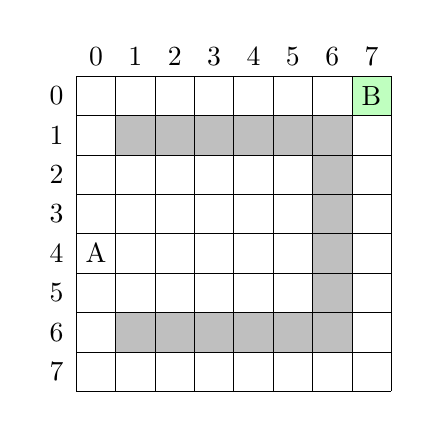
\begin{tikzpicture}
	  			\begin{scope}[xshift=-1.75cm, yshift=1.75cm, xscale=0.5, yscale=0.5]
	\fill[fill = lightgray] (1, -1) 
	  -- ++(6, 0) 
	  -- ++(0, -6) 
	  -- ++(-6, 0) 
	  -- ++(0, 1) 
	  -- ++(5, 0) 
	  -- ++(0, 4) 
	  -- ++(-5, 0) 
	  -- cycle;
	  
	\fill[fill = green!25] (7, -1) -- ++(1, 0) -- ++(0, 1) -- ++(-1, 0) -- cycle;
	
\end{scope}

\begin{scope}[xshift=0.25cm, yshift=-0.25cm]
	\draw[step=0.5cm,black,very thin] (-2,-2) grid (2,2);
\end{scope}

\matrix[matrix, matrix of nodes, nodes={anchor=center,inner sep=0pt,text width=.5cm,align=center,minimum height=.5cm}, nodes in empty cells]{
	& 0 & 1 & 2 & 3 & 4 & 5 & 6 & 7 \\
	0 &   &   &   &   &   &   &   & B \\
	1 &   &   &   &   &   &   &   &   \\
	2 &   &   &   &   &   &   &   &   \\
	3 &   &   &   &   &   &   &   &   \\
	4 & A &   &   &   &   &   &   &   \\
	5 &   &   &   &   &   &   &   &   \\
	6 &   &   &   &   &   &   &   &   \\
	7 &   &   &   &   &   &   &   &   \\};
  			\end{tikzpicture}
  		\end{figure}
  	}{
	  	\begin{itemize}
	  		\item \emph{Provjera rješenja} \engl{goal test} provjerava je li određeno stanje rješenje
	  		\item U slučaju cjelobrojne rešetke, stanje je rješenje ako sadrži "B"
	  	\end{itemize}
    }
  \end{frame}

  \begin{frame}{Trošak prijelaza između stanja}
	\begin{itemize}
      \item \emph{Trošak prijelaza} \engl{step cost} je funkcija koja određuje trošak prijelaza iz stanja \( s \) u stanje \( s' \) akcijom \( a \)
      \item Označava se \( c(s, a, s') \)
	  \item U slučaju cjelobrojne rešetke, trošak prijelaza je \( 1 \) za svako susjedno polje (osim zidova)
    \end{itemize}
  \end{frame}

  \begin{frame}{Heuristička funkcija - definicija}
  	\begin{itemize}
  	  \item \emph{Heuristička funkcija} \engl{heuristic} predstavlja najmanju cijenu puta od stanja \( n \) do stanja koje predstavlja rješenje
  	  \item Označava se \( h(n) \)
  	  \item Za svako stanje \( n \) koje predstavlja rješenje, mora vrijediti \( h(n) = 0 \)
  	\end{itemize}
  \end{frame}

  \begin{frame}{Heuristička funkcija - primjer}
    \twocolumns{
    	\begin{figure}[H]
    		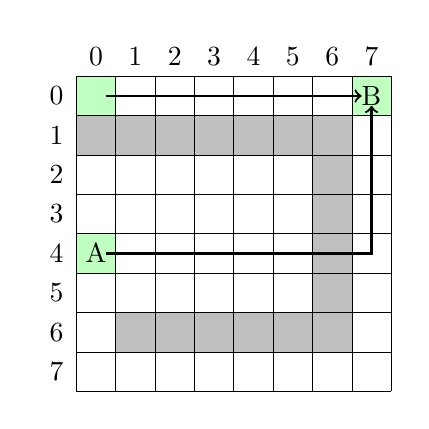
\begin{tikzpicture}
    		\begin{scope}[xshift=-1.75cm, yshift=1.75cm, xscale=0.5, yscale=0.5]
	\fill[fill = lightgray] (0, -1) 
	  -- ++(7, 0) 
	  -- ++(0, -6) 
	  -- ++(-6, 0) 
	  -- ++(0, 1) 
	  -- ++(5, 0) 
	  -- ++(0, 4) 
	  -- ++(-6, 0) 
	  -- cycle;
	  
	\fill[fill = green!25] (7, -1) -- ++(1, 0) -- ++(0, 1) -- ++(-1, 0) -- cycle;
	
	\fill[fill = green!25] (0, -1) -- ++(1, 0) -- ++(0, 1) -- ++(-1, 0) -- cycle;
	
	\fill[fill = green!25] (0, -5) -- ++(1, 0) -- ++(0, 1) -- ++(-1, 0) -- cycle;
\end{scope}

\begin{scope}[xshift=0.25cm, yshift=-0.25cm]
	\draw[step=0.5cm,black,very thin] (-2,-2) grid (2,2);
\end{scope}

\matrix[matrix, matrix of nodes, nodes={anchor=center,inner sep=0pt,text width=.5cm,align=center,minimum height=.5cm}, nodes in empty cells]{
	& 0 & 1 & 2 & 3 & 4 & 5 & 6 & 7 \\
	0 &   &   &   &   &   &   &   & B \\
	1 &   &   &   &   &   &   &   &   \\
	2 &   &   &   &   &   &   &   &   \\
	3 &   &   &   &   &   &   &   &   \\
	4 & A &   &   &   &   &   &   &   \\
	5 &   &   &   &   &   &   &   &   \\
	6 &   &   &   &   &   &   &   &   \\
	7 &   &   &   &   &   &   &   &   \\};

\begin{scope}[xshift=-1.75cm, yshift=1.75cm, xscale=0.5, yscale=0.5]
	\draw [->, thick] (0.75, -0.5) -- ++(6.5, 0);
	\draw [->, thick] (0.75, -4.5) -- ++(6.75, 0) -- ++(0, 3.75);
\end{scope}
    		\end{tikzpicture}
    	\end{figure}
    }{
    	\begin{itemize}
    		\item Jednostavna heuristika za cjelobrojnu rešetku je Manhattan udaljenost između stanja \\[0.5cm]
    	\end{itemize}
    	\[ h(\text{\state{x}{y}}) = |x - x_B| + |y - y_B| \]
    	\[ h(\text{\state{0}{0}}) = 7 \]
    	\[ h(\text{\state{4}{0}}) = 11 \]
    }
  \end{frame}
\end{document}